\documentclass[aspectratio=169]{beamer}\usepackage[utf8]{inputenc}
\usepackage[english]{babel}
\usepackage{color}
\usepackage{amsmath,mathtools}
\usepackage{mathptmx}
\usepackage[11pt]{moresize}
\setbeamertemplate{navigation symbols}{}
\setbeamersize{text margin left=5mm,text margin right=5mm}
\usepackage{wrapfig}
\usepackage{bbm}
\usepackage{xcolor}
\usepackage{tabularx}
\usepackage{bm}


\newcommand{\R}{\mathbb{R}}
\newcommand{\E}{\mathbb{E}}
\newcommand{\N}{\mathbb{N}}
\newcommand{\Z}{\mathbb{Z}}
\newcommand{\V}{\mathbb{V}}
\newcommand{\Q}{\mathbb{Q}}
\newcommand{\K}{\mathbb{K}}
\newcommand{\C}{\mathbb{C}}
\newcommand{\T}{\mathbb{T}}
\newcommand{\I}{\mathbb{I}}

\setbeamertemplate{caption}[numbered]

\title{Inference  Experiments on some Stochastic Differential Equations \\ (miscellaneous toy models)}
\subtitle{ Waleed Alhaddad}

\begin{document}
\setbeamercolor{background canvas}{bg=blue!3}
\begin{frame}
\titlepage
\end{frame}
%
%\begin{frame}\frametitle{Model}
%
%\begin{equation}
%\begin{split}
%dX(t) &= a(X(t); \theta) dt + b (X(t); \theta ) dW(t) \quad t > 0 \\
%X(0) & = x_0
%\end{split}\label{main}
%\end{equation}
%where $X(t) \in [0,1]$ is the normalized stochastic analogue of the power generated $p(t)$. 
%
%\begin{enumerate}
%\item Drift is given by $a(X(t),t ; \theta) = - \theta (t) \Big(X(t)-p(t)\Big)$
%\item Non-centered diffusion is given by: $ b (X(t); \theta) = \sqrt{2\alpha(t) \theta (t) p(t) \Big(1-p(t)\Big) X(t) \Big(1-X(t)\Big)}  $
%\end{enumerate}
%
%\end{frame}


%\begin{frame}[label=guide]\frametitle{ Reader's Guide }
%
%List of changes in this iteration:
%\begin{itemize}
%\item Matched data with every forecast
%\item Normalized according to installed power of each period
%\item Interpolated the forecast using cubic splines.
%
%\end{itemize}
%
%Next steps:
%\begin{itemize}
%\item upgrade the numerical integrator and use the interpolated forecast
%\item Check performace using the interpolated forecasts and data
%\end{itemize}
%
%Note :
%\begin{itemize}
%\item Green slides: possible future extensions
%\item Red slides: notes to be removed
%\end{itemize}
%
%\end{frame}


\begin{frame}\frametitle{ Toy models }
We generate paths from an SDE  with given parameters and then fit the model to check the retrievability of the parameters. We consider the following cases:
\begin{itemize}
\item[1:]  Constant parameter Wiener process: finite and infinite horizon.
\item[2:]  Controlled Wiener process within an interval.
\item[3:]  Controlled Wiener process centered around a given function. 
\end{itemize}
\end{frame}


\begin{frame}\frametitle{ Stochastic Differential Equation }
Given the SDE
\begin{equation}
\begin{split}
dX_t &= a(X_t; \bm{\theta}) dt + b (X_t; \bm{\theta} ) dW_t \quad t > 0 \\
X_0 & = x_0
\end{split}\label{main}
\end{equation}
Consider a set of N observations, $ X=\{ X_{t_0^N} , X_{t_1^N} ,\ldots , X_{t_N^N} \}$ observed within intervals $\Delta_N$. 

\begin{itemize}
\item $\Delta_N$: is any function of the number of samples, $N$. For example, $\Delta_N = \frac{1}{N}$.
\item $a(X_t; \bm{\theta})$ is the drift function \textcolor{brown}{(add technical conditions here)}
\item $b (X_t; \bm{\theta} )$ is the diffusion function \textcolor{brown}{(add technical conditions here)}
\item $\bm{\theta}$ is a vector of constant parameters
\end{itemize}
\end{frame}

\begin{frame}\frametitle{ likelihood function }
We have the Likelihood function of the transition density

\begin{equation}
\mathcal{L}(\theta;X) = \prod\limits_{i=1}^n\rho( {X_{i+1}|X_{i}}, \bm{\theta})  \rho(X_0) 
\end{equation}
Consider a Gaussian transition density,
\begin{equation*}
\mathcal{L}(\bm{\theta}; X) = \prod\limits_{i=1}^n  \frac{1}{\sqrt{2 \pi b(X_i,\bm{\theta})^2 dt}  } \exp\Big(\frac{-((X_{i+1}-X_i) - a(X_i,\bm{\theta}) dt )^2}{2b(X_i,\bm{\theta})^2 dt}\Big) \rho(X_0)
\end{equation*}

We take the improper prior $\rho(X_0)=1$.
\end{frame}

\begin{frame}\frametitle{ Case 1: Constant Parameters }
For a fixed $b(X_t; \bm{\theta})=\sigma$ and a fixed $a(X_t; \bm{\theta})=\mu$. We observe that varying the sampling and discretization parameters affects the convergence behavior.


We consider the following three situations:
\begin{enumerate}
\item[1.1] Infinite Horizon expansion caused by increasing samples N\\ ( increasing $N$ and $\Delta_N$ is fixed).
\item[1.2] Infinite Horizon expansion caused by increasing intervals $\Delta_N$ \\ ( fixed $N$ and increasing decreasing $\Delta_N$).
\item[1.3] Finite Horizon expansion with sample compression, i.e where $\Delta_N=\frac{T}{N}$ \\ (increasing $N$, fixed $T$).
\end{enumerate}
\end{frame}


\begin{frame}\frametitle{ Case 1: Implementation }

In the following, we use  L-BFGS-B algorithm to optimize the likelihood with bounds on $\sigma$ being positive. And we use $\mu=100$ and $\sigma=10$ for the path generation. We denote the estimators of $\mu$ and $\sigma$ by  $\hat{\mu}$ and $\hat{\sigma}$ where,

\begin{equation}
 \hat{\mu} = \arg \underset{\mu \in \R}{\max} \ \mathcal{L}(\bm{\theta};X) \quad \quad  \quad \quad \hat{\sigma} = \arg \underset{\sigma \in \R^+}{\max} \mathcal{L}(\bm{\theta};X)
\end{equation}

\end{frame}


\begin{frame}%\frametitle{ Case 1: Scenario illustration }
The above cases can be seen clearly in the illustration below.
\begin{figure}
  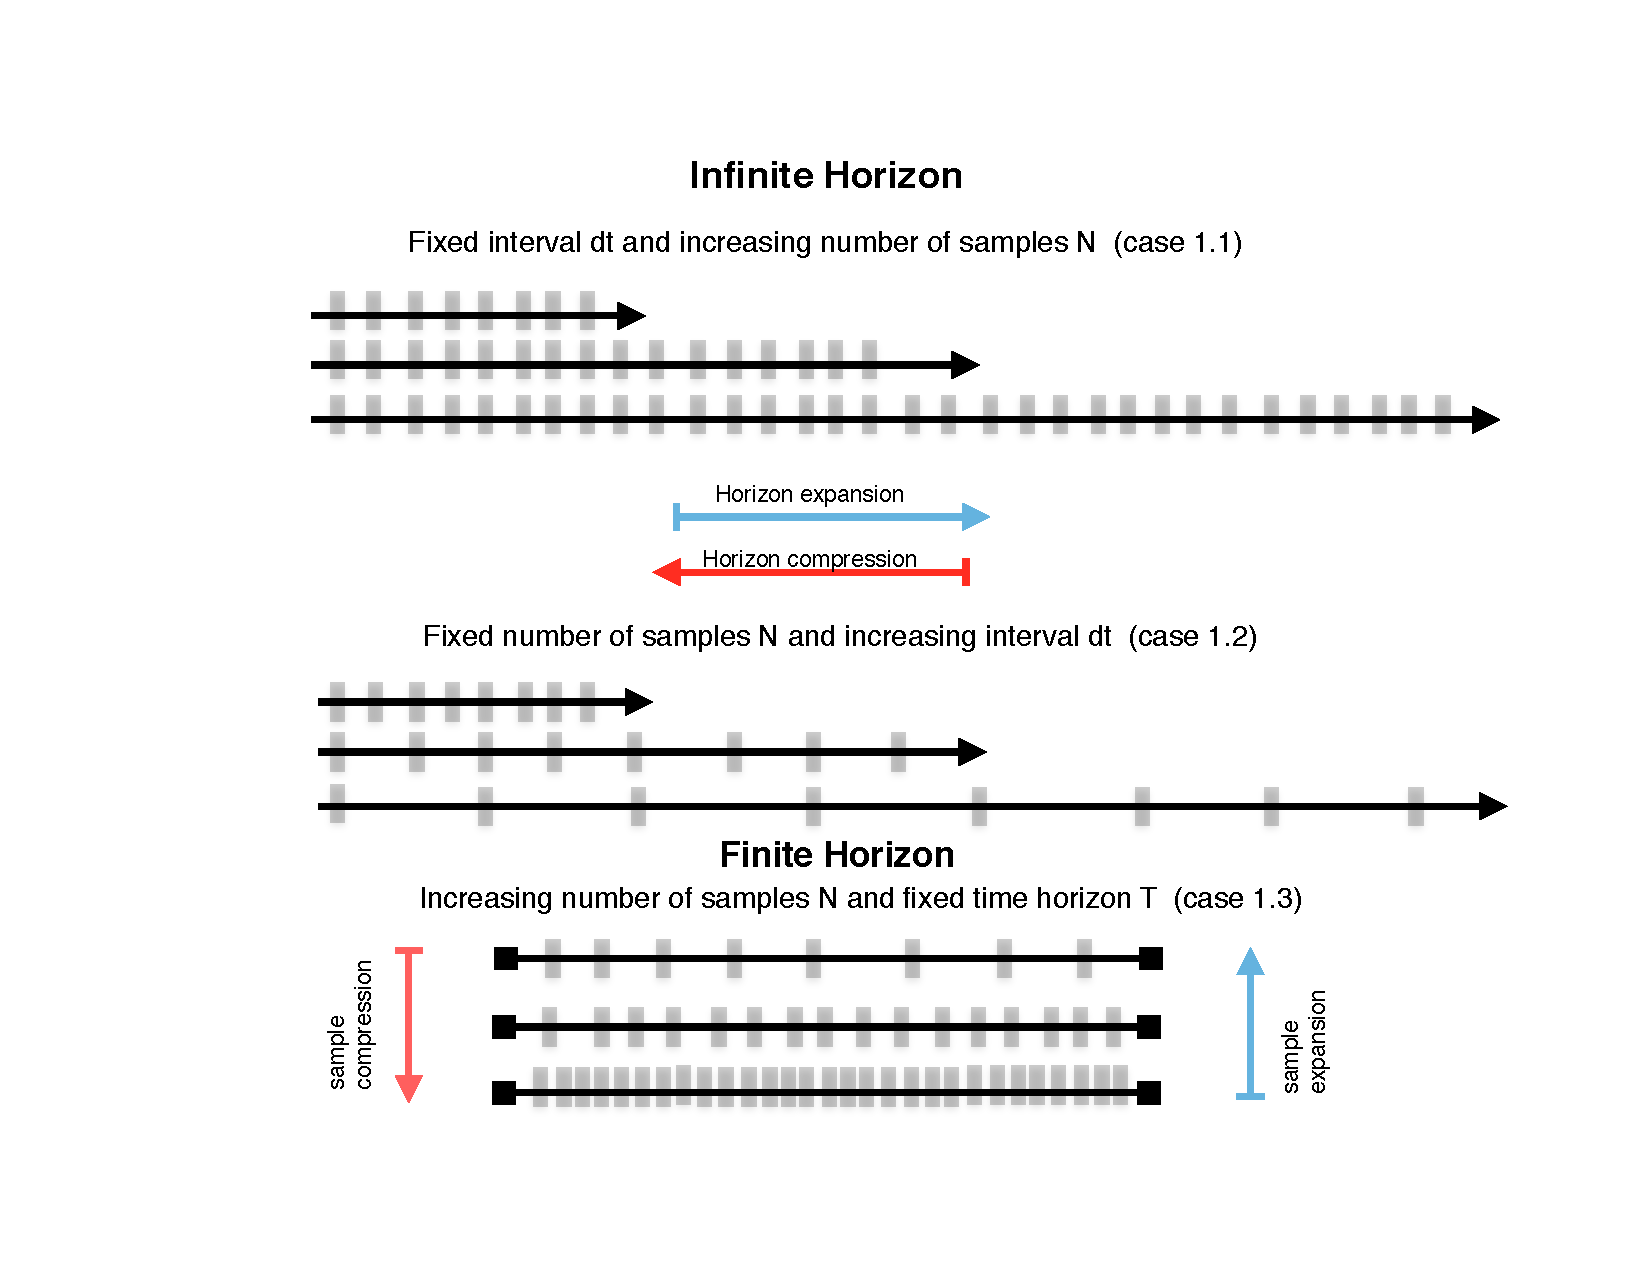
\includegraphics[scale=0.4]{Figures/data_horizons.pdf}
  %\label{fig:boat1}
\end{figure}
\end{frame}





%\begin{itemize}
%\item $ \sigma (X(t); \theta) = \sqrt{2 p(t) \Big(1-p(t)\Big) X(t) \Big(1-X(t)\Big)}  $
%\item $b(X(t),t ; \theta) = -  \Big(X(t)-p(t)\Big)$
%\end{itemize}

\begin{frame}\frametitle{ Case 1.1: Constant Parameters \\
 Infinite Horizon expansion caused by increasing samples N }
An increase of the number of samples $N$ in a growing time interval $T$. In this case, we obtain  convergence of the order $\frac{1}{\sqrt{N}}$ as expected.

\begin{figure}
  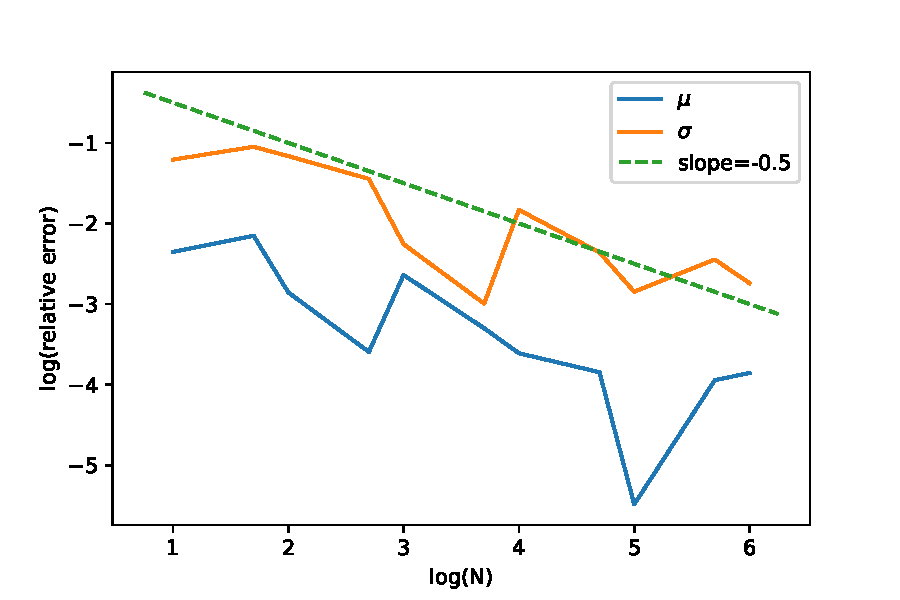
\includegraphics[scale=0.45]{Figures/case11v2.pdf}
  \caption{convergence in the case of infinite horizon expansion caused by increasing samples N}
  %\label{fig:boat1}
\end{figure}

\end{frame}

\begin{frame}\frametitle{ Case 1.2: Constant Parameters \\
 Infinite Horizon expansion caused by increasing intervals dt }
In this case, the estimator $\hat{\sigma}$ of the diffusion coefficient is inconsistent. This is because the time interval between the samples is increasing and so we do not have as much information about the variation of the process. However, the drift estimator $\hat{\mu}$ is still consistent. We have not seen any theoretical proof of this situation.

\begin{figure}
  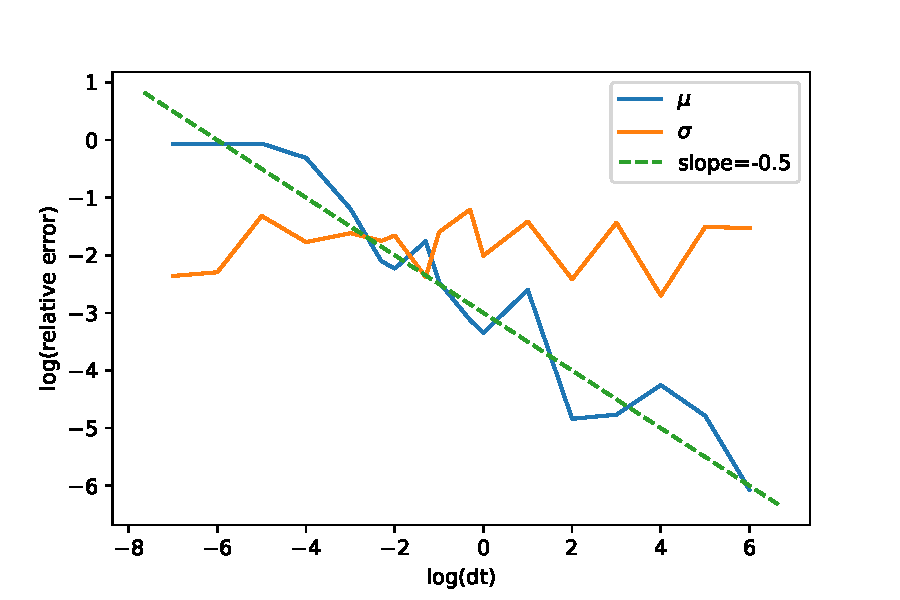
\includegraphics[scale=0.45]{Figures/case12v3.pdf}
  \caption{convergence rate in the case of infinite horizon expansion caused by increasing intervals $\Delta_N$}
  %\label{fig:boat1}
\end{figure}

\end{frame}


\begin{frame}\frametitle{ Case 1.3: Constant Parameters \\
 Finite Horizon expansion with sample compression }
In this case, we observe increasing number of  samples in a fixed time interval (sample compression).In this case the drift estimator $\mu$ is inconsistent while the diffusion estimator $\sigma$ is consistent. This situation  matches the theoretical discussion in [1].

\begin{figure}
  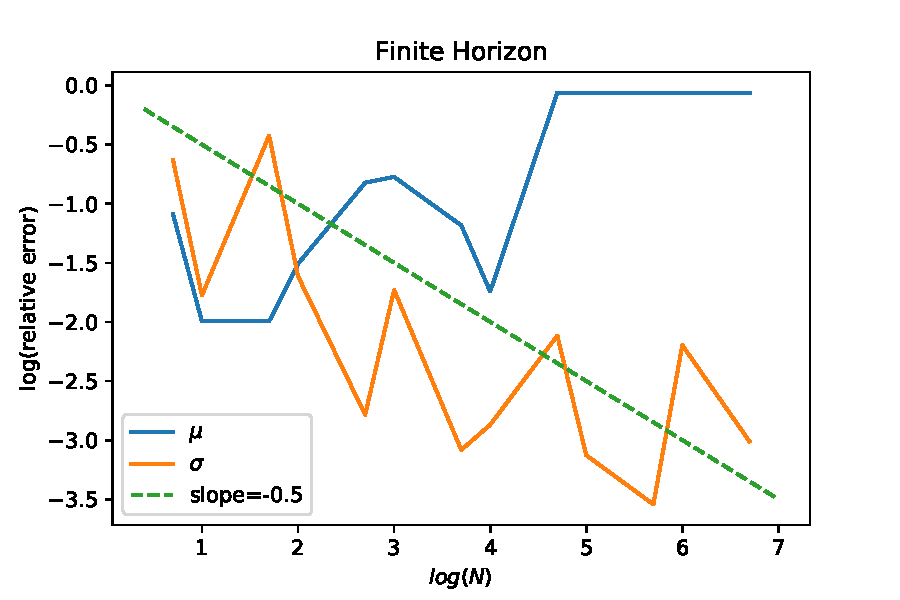
\includegraphics[scale=0.45]{Figures/case13v2.pdf}
  \caption{Convergence rate in the case of finite horizon expansion with sample compression  }
  %\label{fig:boat1}
\end{figure}

We will see next that there are no consistent estimators of the drift  term $b(X(t), \theta)$ in this case. 

\end{frame}


\begin{frame}\frametitle{ Remarks }
\begin{enumerate}
\item  It is easier to obtain convergence in the diffusion coefficient. Because the estimator of the diffusion has access to  information from the infinite variation of the wiener process while the drift does not. We can show this theoretically from the efficiency condition of the estimators.
\item The convergence generally follows Monte Carlo's convergence rate in terms of sampling as expected. This statement is wrong in a high frequency setting, as we have different convergence rate for estimator of the diffusion and than for the estimator of the drift as we will see next. The estimator of the drift converges slower than the Monte Carlo rate given that both are consistent.
\end{enumerate}

\end{frame}

\begin{frame}\frametitle{Motivation of high frequency SDE data}

High frequency situations are not uncommon and extreme  but may happen for data that looks reasonable. For instance, in some cases  weekly data is treated as high frequency data . A situation is considered high frequency with respect to the amount of  variation in the drift term [1] (or in regards to the speed at which it reverts to the mean).  \\

This also important for building confidence intervals as the limiting distribution of our estimator may not be Gaussian. For example, in the setting of high frequency data and fixed time $T$ (case 1.3 above) the limiting distribution of the estimator is path dependent and is given by a normal variance-mixture distribution which can be heavy tailed with no finite moments [1]. However, in this case, a  modification of the estimator can help in achieving  a Gaussian limiting distribution of the estimator.

Please note that in the setting of high frequency SDE data, we have two possibilities:
\begin{itemize}
\item Finite Horizon (fixed time $T$): this corresponds to case 1.3 above.
\item Infinite Horizon: this corresponds to other two cases.
\end{itemize}


\end{frame}

\begin{frame}\frametitle{Convergence of the drift estimator for high frequency  SDE  \\(Case 1.3 / Finite Horizon)}

In a high frequency setting with finite horizon (case 1.3), there are \textbf{no} consistent estimators of the drift term $a(X_t, \bm{\theta})$ (see [1]) as we break the following condition :\\

Given the following SDE,
\begin{equation}
\begin{split}
dX_t &= a(X_t; \alpha) dt + b(X_t; \beta ) dW_t \quad t > 0 \\
X(0) & = x_0
\end{split}\label{main}
\end{equation}

the drift estimator  $\hat{\alpha}$ of the parameter set $\alpha$ of the system is consistent if and only if
\begin{equation}
n \Delta_n \to \infty  \label{conv_cond}
\end{equation}
And this condition contradicts having a finite horizon as we trivially have $T=N \Delta_N \to \infty$. If the  condition (\ref{conv_cond}) is not satisfied, we cannot have a consistent estimator  $\hat{\alpha}$ of the drift. However, the estimator $\hat{\beta}$ of the diffusion term $b (X_t; \beta)$ is still consistent regardless. 
\end{frame}



\begin{frame}\frametitle{Convergence of the drift estimator for high frequency  SDE  \\(Case 1.3 / Finite Horizon)}
To show this result numerically, we pick any $\Delta_n$ such that $T=n \Delta_n \to \infty$. In this example, we modify the non-consistent  drift parameter estimator (case $1.3$) such that 
\begin{equation}
dt=\frac{T}{N} \quad  \rightarrow  \quad dt=\frac{T}{\sqrt{N}}
\end{equation}
Then we recover back the convergence of the other cases as this replacement turns the finite horizon to an infinite horizon. 
\end{frame}


\begin{frame}\frametitle{Numerical Convergence for high frequency  SDE}
In this numerical example, we take $\Delta_N = \frac{T}{\sqrt{N}}$ as an example.
\begin{equation}
\text{Finite Horizon:} \ dt=\frac{T}{N} \quad  \text{versus} \quad \text{Infinite Horizon:} \ dt=\frac{T}{\sqrt{N}}
\end{equation}
We confirm  condition (\ref{conv_cond}) numerically. It is clear that in the finite horizon case the estimator of the diffusion $\hat{\sigma}$ converges while the estimator of the drift $\hat{\mu}$ is not consistent. Whereas, in the infinite horizon case, we obtain the expected convergence in both parameters.
\begin{figure}
  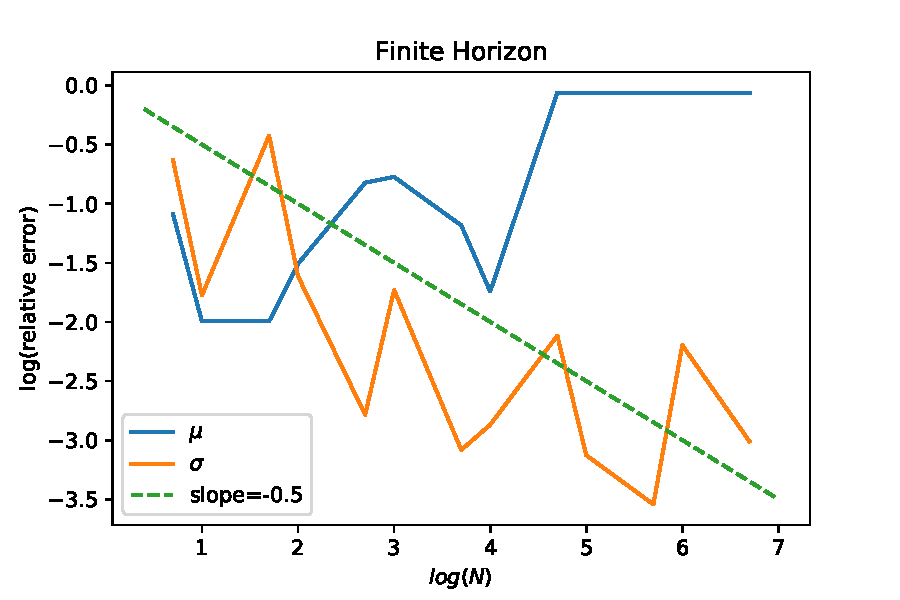
\includegraphics[scale=0.35]{Figures/case13v2.pdf}
   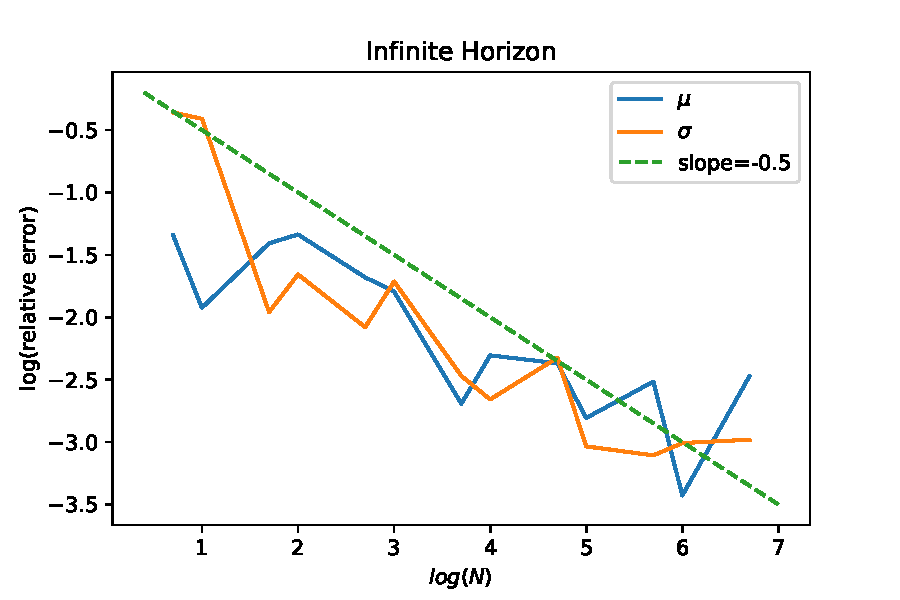
\includegraphics[scale=0.35]{Figures/case13infinite.pdf}
  \caption{Right side: Finite horizon with $dt=\frac{T}{N}$, Left side: Infinite horizon with $dt=\frac{T}{\sqrt{N}}$   }
  %\label{fig:boat1}
\end{figure}

\end{frame}





\begin{frame}\frametitle{Convergence for high frequency SDE data}
We can show that the score function of the likelihood is an efficient martingale estimating function and that the obtained estimator is optimal\footnote{If we consider an approximate martingale estimator function such as the pseudo likelihood, then we require an extra condition that $n \Delta_n^{2 \kappa - 1} \to 0 $ where $\kappa$ is the order of $\Delta_N$ in RHS of the expectation (\ref{expec_martin})}. Then we have the following convergence rates [3]:

For a finite Horizon (fixed T)
\begin{equation}
\hat{\alpha} \text{ is not consistent } \quad \text{and} \quad relative \ error(\hat{\beta}) \propto \frac{1}{\sqrt{N}}
\end{equation}
For an infinite Horizon ($T \to \infty$)
\begin{equation}
relative \ error(\hat{\alpha})  \propto \frac{1}{\sqrt{N\Delta_N}} \quad \text{and} \quad  relative \ error(\hat{\beta}) \propto \frac{1}{\sqrt{N}} 
\end{equation}
Note that the estimator $\hat{\alpha}$ of the drift is affected by the time discretization while the estimator $\hat{\beta}$ of the diffusion is independent of the time discretization.

\end{frame}


\begin{frame}\frametitle{High Frequency  SDE General Convergence }
Consider a set of N observations, $X= \{ X_{t_0^N} , X_{t_1^N} ,\ldots , X_{t_N^N} \}$ and the following martingale estimator function,
\begin{equation}
G_n(\gamma) = \sum\limits_{i=1}^N g(\Delta_N , X_{t_{i}^N},X_{t_{i-1}^N} ; \gamma )
\end{equation}
where $t_{i}^n = i \Delta_n $, $\gamma = (\alpha, \beta)$ and $g=(g_1, g_2)$ .
In our martingale case\footnote{The results can also be adapted to a non martingale estimating function such as a pseudo likelihood},we must have,
\begin{equation}
E_\gamma \Big(    g(\Delta_N , X_{t_{i}^N},X_{t_{i-1}^N} ; \gamma) \Big| X_{t_{i-1}^N}  \Big) = 0
\label{expec_martin}
\end{equation} where the $\hat{\beta}$ estimator is given by solving $ G_n(\gamma) = 0 $.

\end{frame}

{
%\setbeamercolor{background canvas}{bg=green!30}

%\begin{frame}\frametitle{High Frequency  SDE -  Possible Extensions}
%
%\begin{itemize}
%\item Try to understand the limit of when we need to switch to the high frequency from the low frequency regime. That is how it depends on the speed of the  mean reversion in our model.
%\item Get the martingale estimator function of the Gaussian transition density explicitly.
%\item State the optimality and efficiency of the estimators explicitly.
%\item Obtain the stated theoretical convergence rate.
%\item Try to show theoretically why in case 1.2 , the diffusion estimator is not consistent.
%\item Understand and state the conditions under which we have a unique parameter estimation to our SDE.
%\end{itemize}
%
%\end{frame}
%}


\begin{frame}\frametitle{References}
\begin{itemize}
\item[][1] Jakobsen, N. M., \& Sørensen, M. (2017). Efficient estimation for diffusions sampled at high frequency over a fixed time interval. Bernoulli, 23(3), 1874-1910. doi:10.3150/15-bej799
\item[][2] Sørensen, M. (2007). Efficient Estimation for Ergodic Diffusions Sampled at High Frequency. SSRN Electronic Journal. doi:10.2139/ssrn.1150694
\item[][3] Kessler, M., Lindner, A., \& Sørensen, M. (2012). Statistical methods for stochastic differential equations. Boca Raton, FL: Chapman \& Hall/CRC.
\end{itemize}

\end{frame}


\begin{frame}\frametitle{ Paths as IID samples  }

We have the Likelihood function of the transition density

\begin{equation}
\mathcal{L}(\theta;X) = \prod\limits_{j=1}^M\prod\limits_{i=1}^N\rho( {X_{j,i+1}|X_{j,i}}, \bm{\theta})  \rho(X_0) 
\end{equation}
Consider a Gaussian transition density,
\begin{equation*}
\mathcal{L}(\bm{\theta}; X) = \prod\limits_{j=1}^M \prod\limits_{i=1}^N  \frac{1}{\sqrt{2 \pi b(X_{j,i};\bm{\theta})^2 dt}  } \exp\Big(\frac{-((X_{j,i+1}-X_{j,i}) - a(X_{j,i};\bm{\theta}) dt )^2}{2b(X_{j,i};\bm{\theta})^2 dt}\Big) \rho(X_0)
\end{equation*}

We take the improper prior $\rho(X_0)=1$.

\end{frame}

\begin{frame}\frametitle{ Paths as IID samples - Implementation }

As before, we use  L-BFGS-B algorithm to optimize the likelihood with bounds on $\sigma$ being positive. We denote the estimators of $\mu$ and $\sigma$ by  $\hat{\mu}$ and $\hat{\sigma}$ where,

\begin{equation}
 \hat{\mu} = \arg \underset{\mu \in \R}{\max} \ \mathcal{L}(\bm{\theta};X) \quad \quad  \quad \quad \hat{\sigma} = \arg \underset{\sigma \in \R^+}{\max} \mathcal{L}(\bm{\theta};X)
\end{equation}

\end{frame}

\begin{frame}\frametitle{ Paths as IID samples - Convergence }
We have Monte Carlo convergence in terms of samples as expected.
\begin{figure}
  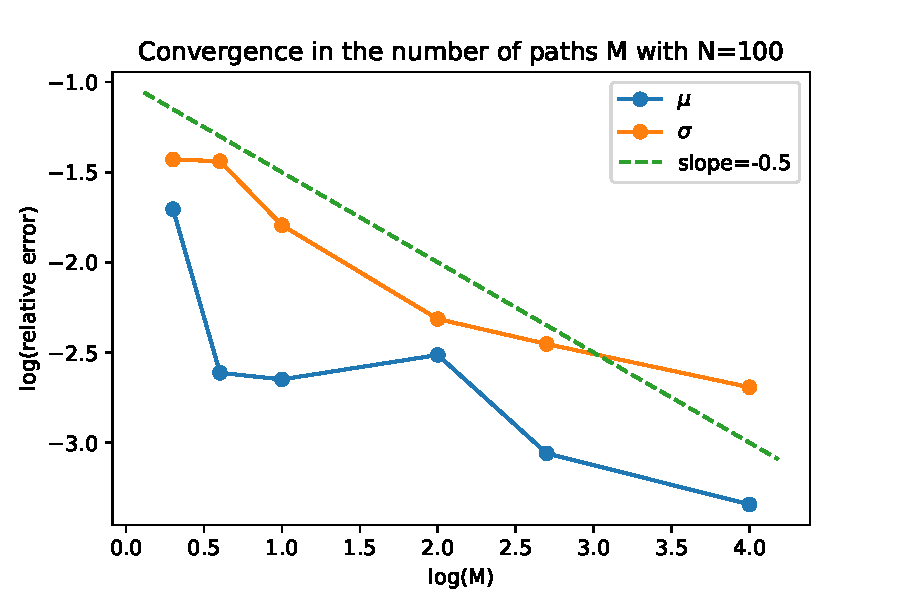
\includegraphics[scale=0.5]{Figures/conv_M_unbounded.pdf}
   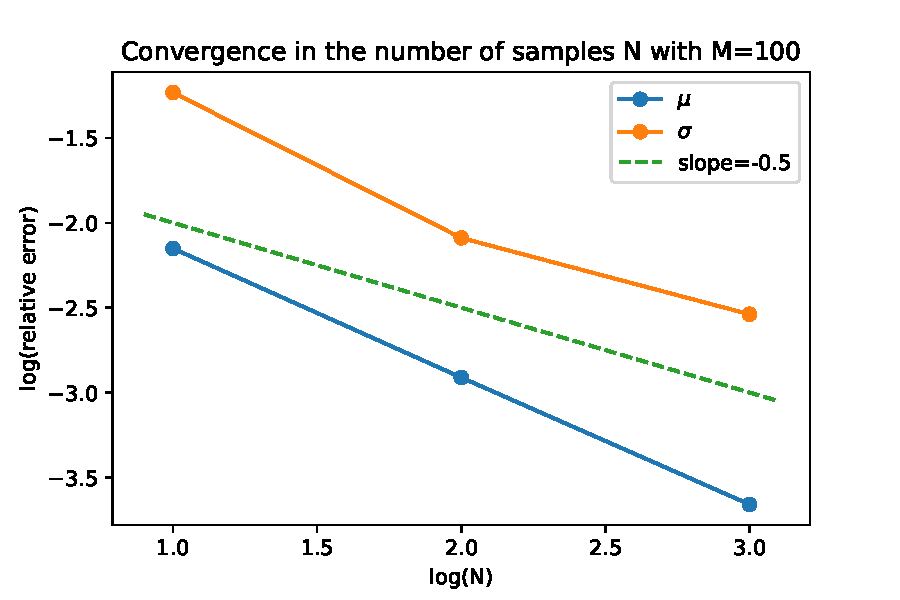
\includegraphics[scale=0.5]{Figures/conv_N_unbounded.pdf}
  \caption{ Optimized using L-BFGS-B algorithm. True parameters used are $\mu = 100$ and $\sigma = 10$.M is the number of paths and N is the number of samples.    }
  %\label{fig:boat1}
\end{figure}

\end{frame}



\begin{frame}\frametitle{Case 2: Controlled Wiener process in a unit box }
We have the SDE,
\begin{equation}
\begin{split}
dX_t &= a(X_t; \bm{\theta}) dt + b (X_t; \bm{\theta} ) dW_t \quad t > 0 \\
X_0 & = 0
\end{split}\label{main}
\end{equation}
Consider a set of N observations, $X= \{ X_{t_0^N} , X_{t_1^N} ,\ldots , X_{t_N^N} \}$ on intervals of $\Delta_N$.\\ We choose,
\begin{equation}
a_{i+1}(X_i; \bm{\theta})= \mu X_i(\frac{1}{2} - X_i)  \quad \quad b_{i+1} (X_i; \bm{\theta} )=\sigma X_i (1-X_i)
\end{equation}
We choose $ 0<\sigma <<1$ and $\mu\in (0,1]$. Then, we have contained the Wiener process in the interval $[0,1]$ with high probability.

\end{frame}


\begin{frame}\frametitle{Case 2: Controlled Wiener process in a unit box }
We see that the process is contained within the unit box as we kill the diffusion coefficient if we touch the boundary. Additionally, the drift coefficient is always directed towards the center line $\frac{1}{2}$ of the unit box.
\begin{figure}
  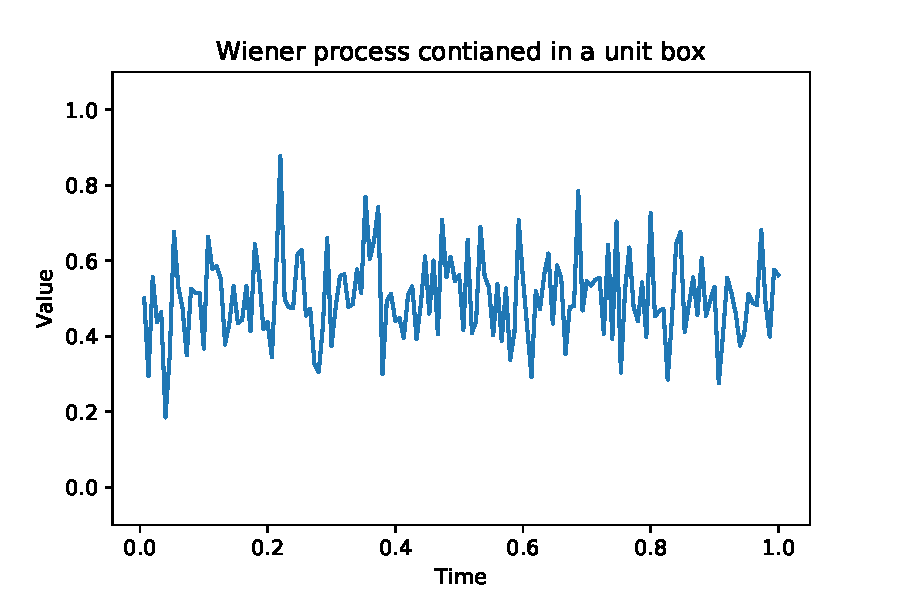
\includegraphics[scale=0.45]{Figures/Wiener_box.pdf}
  \caption{ With  high probability the wiener process stays inside the box as $\mu \in (0,1]$ and $\sigma << 1$ }.
  %\label{fig:boat1}
\end{figure}

\end{frame}


\begin{frame}\frametitle{Case 2: Controlled Wiener process in a unit box - Parameter Inference }

We obtain the same convergence as before,

\begin{figure}
  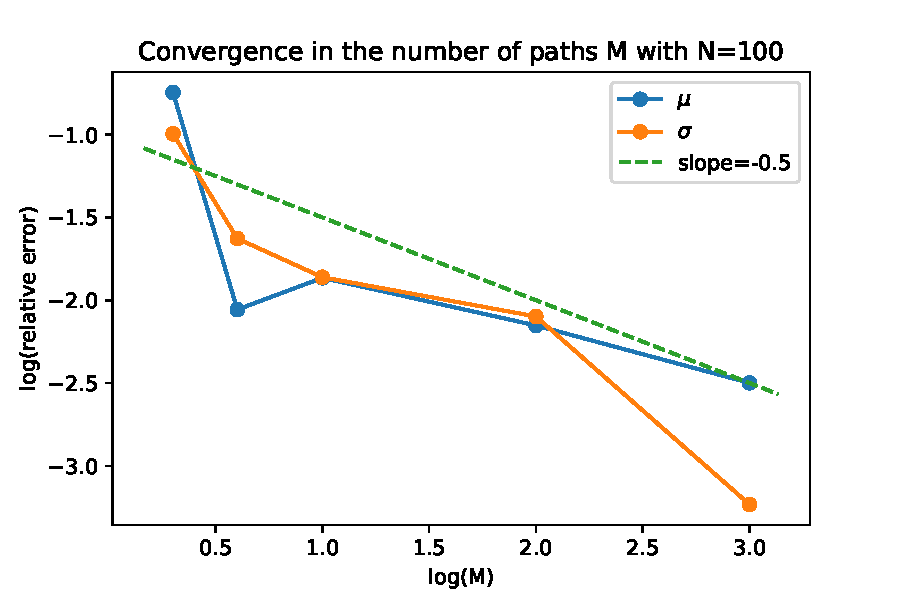
\includegraphics[scale=0.5]{Figures/conv_M_box.pdf}
   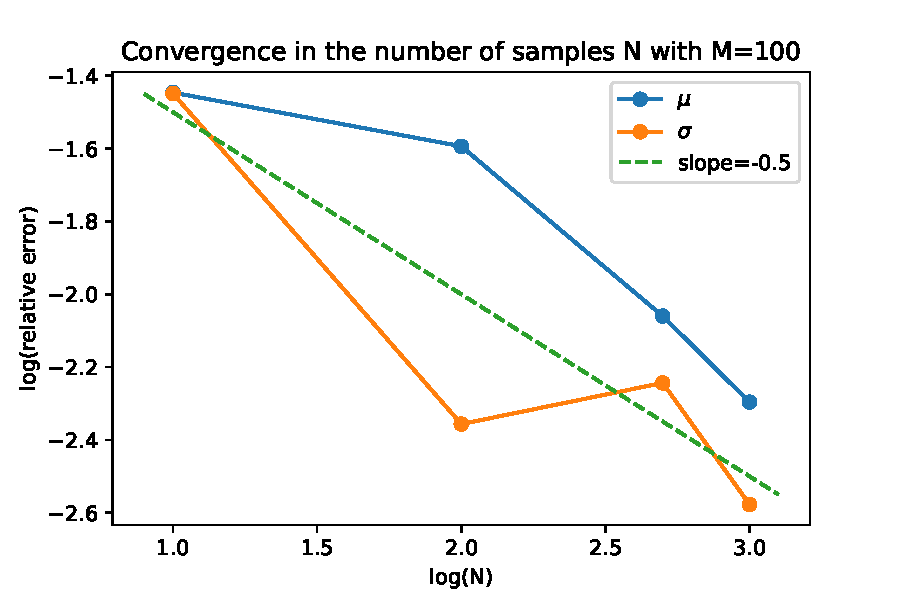
\includegraphics[scale=0.5]{Figures/conv_N_box.pdf}
  \caption{Optimized using L-BFGS-B algorithm. True parameters used are $\mu = 0.5$ and $\sigma = 0.1$. M is the number of paths and N is the number of samples.   }
  %\label{fig:boat1}
\end{figure}

\end{frame}


\begin{frame}\frametitle{Case 3: Controlled Wiener process around a given function }
We have the SDE,
\begin{equation}
\begin{split}
dX_t &= a(X_t; \bm{\theta}) dt + b (X_t; \bm{\theta} ) dW_t \quad t > 0 \\
X_0 & = 0
\end{split}\label{main}
\end{equation}
Consider a set of N observations, $X= \{ X_{t_0^N} , X_{t_1^N} ,\ldots , X_{t_N^N} \}$ on intervals of $\Delta_N$.\\ We choose,
\begin{equation}
a_{i+1}(X_i; \bm{\theta})= \mu X_i(\frac{1}{2}(1 + p_i )- X_i)  \quad \quad b_{i+1} (X_i; \bm{\theta} )=\sigma X_i (1-X_i)
\end{equation}
We choose $ 0<\sigma <<1$ and $\mu\in (0,1]$. Then, we have contained the Wiener process in the interval $[0,1]$ with high probability. Additionally, we add mean reversion to $\frac{1}{2}(1 + p_i ) $ where  $p_i = \sin(\frac{i}{N} 2\pi)$.


\end{frame}

\begin{frame}\frametitle{Case 3: Controlled Wiener process following a given function }
We see that the process follows the sine wave  closely when the  drift parameter $\mu \approx 1$ and that we have a shift artifact when the drift parameter $\mu<<1$. Note that the process does not  escape the unit box as the diffusion is controlled and the drift is directed towards the function which is always inside the unit box.
\begin{figure}
  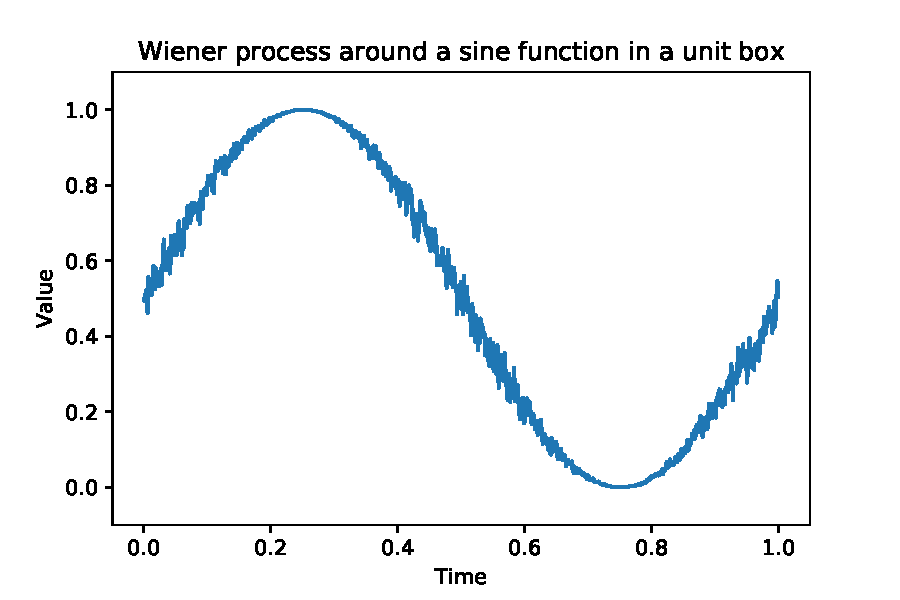
\includegraphics[scale=0.4]{Figures/Wiener_sine_box.pdf}
   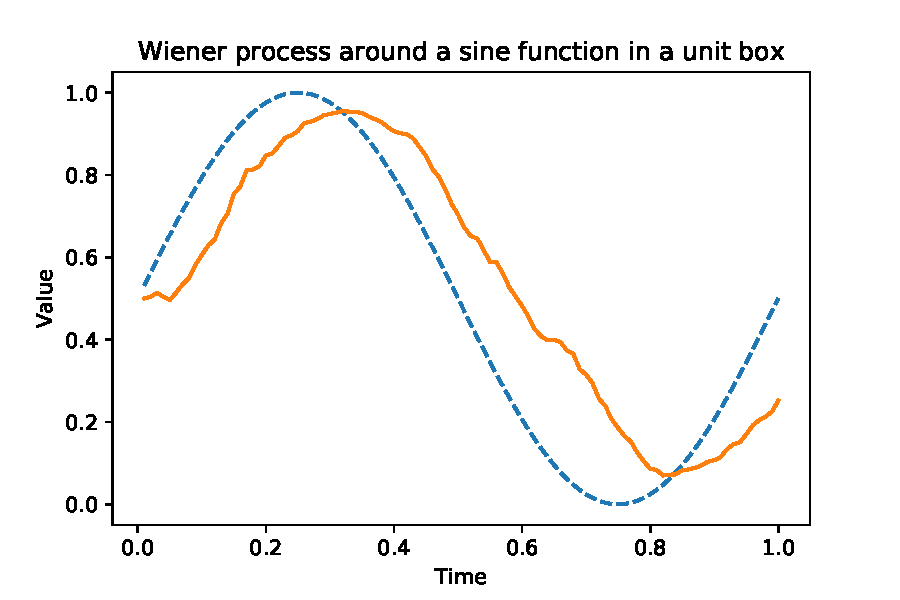
\includegraphics[scale=0.4]{Figures/conv_sine_shift.pdf}
  \caption{Illustrative examples: On the right, we see the controlled wiener process responding to the boundary  by killing the diffusion at the peaks of the sine wave. On the right we observe an unintended  shift artifact when the drift parameter $\mu<<1$.   }
  %\label{fig:boat1}
\end{figure}

\end{frame}

\begin{frame}\frametitle{Case 3: Controlled Wiener process around a function - Paramter Inference }
We obtain the same convergence as before,

\begin{figure}
  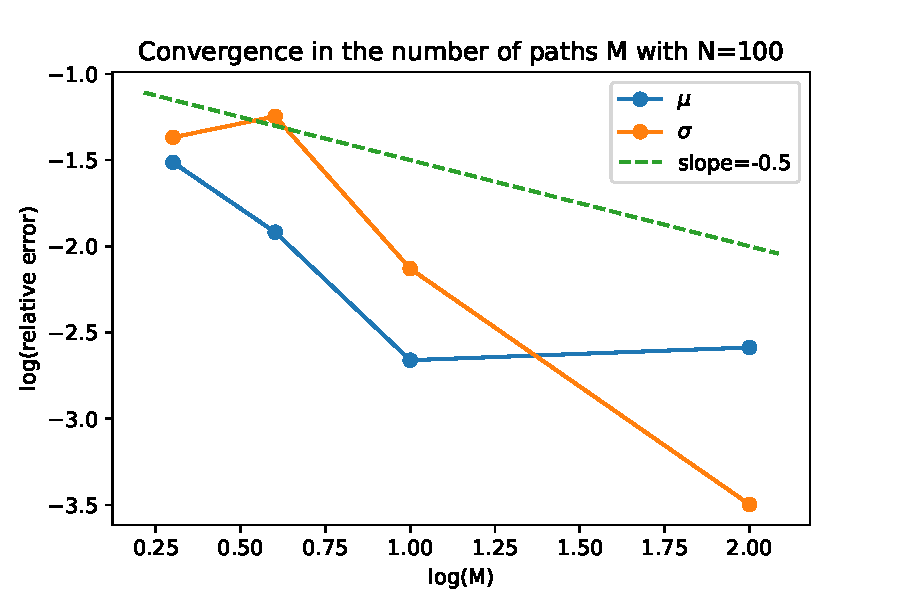
\includegraphics[scale=0.5]{Figures/conv_M_sine.pdf}
   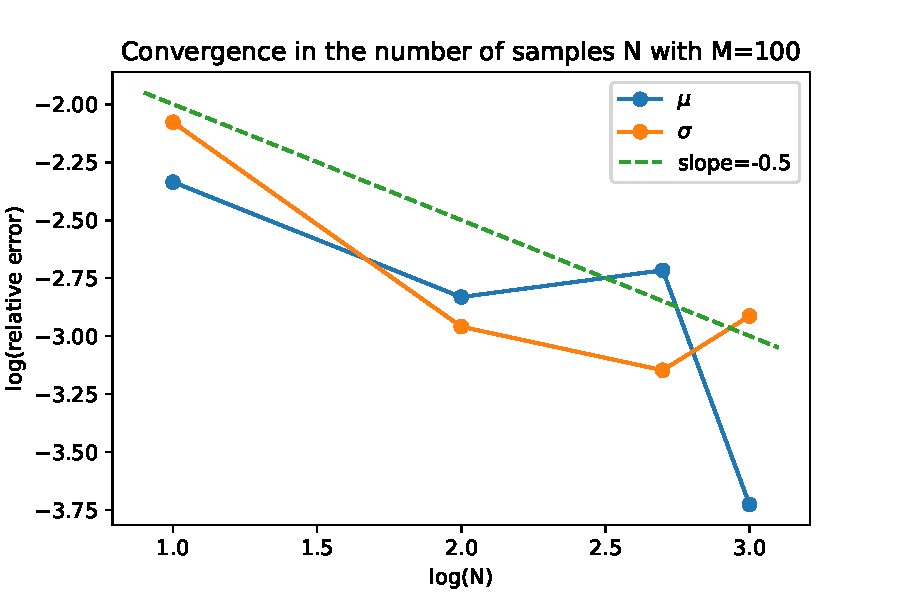
\includegraphics[scale=0.5]{Figures/conv_N_sine.pdf}
  \caption{ Optimized using L-BFGS-B algorithm. True parameters used are $\mu = 100$ and $\sigma = 10$.M is the number of paths and N is the number of samples.    }
  \label{fig:sine}
\end{figure}

\end{frame}






%\againframe{guide}



\end{document}






























